% ****** Start of file apssamp.tex ******
%
%   This file is part of the APS files in the REVTeX 4.2 distribution.
%   Version 4.2a of REVTeX, December 2014
%
%   Copyright (c) 2014 The American Physical Society.
%
%   See the REVTeX 4 README file for restrictions and more information.
%
% TeX'ing this file requires that you have AMS-LaTeX 2.0 installed
% as well as the rest of the prerequisites for REVTeX 4.2
%
% See the REVTeX 4 README file
% It also requires running BibTeX. The commands are as follows:
%
%  1)  latex apssamp.tex
%  2)  bibtex apssamp
%  3)  latex apssamp.tex
%  4)  latex apssamp.tex
%
\documentclass[%
 reprint,
%superscriptaddress,
%groupedaddress,
%unsortedaddress,
%runinaddress,
%frontmatterverbose, 
%preprint,
%preprintnumbers,
%nofootinbib,
%nobibnotes,
%bibnotes,
 amsmath,amssymb,
 aps,
%pra,
%prb,
%rmp,
%prstab,
%prstper,
%floatfix,
]{revtex4-2}

\usepackage{booktabs}
\usepackage{graphicx}% Include figure files
\usepackage{dcolumn}% Align table columns on decimal point
\usepackage{bm}% bold math
\usepackage{enumitem}
\usepackage[mathlines]{lineno}% Enable numbering of text and display math
%\linenumbers\relax % Commence numbering lines

%\usepackage[showframe,%Uncomment any one of the following lines to test 
%%scale=0.7, marginratio={1:1, 2:3}, ignoreall,% default settings
%%text={7in,10in},centering,
%%margin=1.5in,
%%total={6.5in,8.75in}, top=1.2in, left=0.9in, includefoot,
%%height=10in,a5paper,hmargin={3cm,0.8in},
%]{geometry}
\usepackage[english, spanish, mexico, es-noitemize]{babel}
\usepackage[pdfusetitle, colorlinks]{hyperref}
\hypersetup{
    colorlinks=true,    % Colores en lugar de cajas
    linkcolor=gray,
    citecolor=black, % Color de los enlaces internos
    filecolor=gray,  % Color de los enlaces a archivos
    urlcolor=gray       % Color de los enlaces externos
}
%\usepackage[shortlabels, inline]{enumitem}
\usepackage{array}
%\usepackage{titlesec}
%\usepackage[titles]{tocloft}
%\usepackage{xcolor, xpatch, calc}
%\usepackage{graphicx, booktabs}
%\usepackage{pgfplots}
%\usepackage[outline]{contour}
%\usepackage[hang, labelfont=bf, labelsep=period, margin=0.5in]{caption}
\usepackage{subcaption}
%\usepackage{csquotes}
\usepackage{lipsum}
%\usepackage{blindtext}
\usepackage{amsmath}
\usepackage{graphicx}
%\usepackage{svg}
%\usepackage{booktabs}
%\usepackage{enumitem}
\usepackage{float}
\usepackage{listings}
\usepackage{xcolor}
\usepackage{listings}
\lstset{
  language=Python,
  basicstyle=\ttfamily\small,
  commentstyle=\itshape\color{gray},
  keywordstyle=\bfseries\color{blue},
  numbers=left,
  numberstyle=\tiny\color{gray},
  stepnumber=1,
  numbersep=5pt,
  backgroundcolor=\color{white},
  frame=single,
  breaklines=true,
  breakatwhitespace=false,
  captionpos=b,
  tabsize=2,
  showspaces=false,
  showstringspaces=false
}

\usepackage{appendix}


\begin{document}

\preprint{APS/123-QED}

\title{Emisión Termoionica}% Force line breaks with \\

 
\author{Grupo 5: J. Gutiérrez}
\email{jgutierrezco@unal.edu.co}
\author{J. Mayorga}
\email{jmayorgab@unal.edu.co}
\author{J. Segura}
\email{jusegurag@unal.edu.co}
\affiliation{Experimentos en Física Moderna [2016687]\\Universidad Nacional de Colombia\\ Departamento de Física - Bogotá D.C}%
\date{\today}% It is always \today, today,
             %  but any date may be explicitly specified
\begin{abstract}
\begin{description}
\item[Resumen] En este trabajo se comprobarán la ley de Child, que describe la densidad de corriente eléctrica que pasa por un diodo en relación al potencial entre cátodo y ánodo; la ley de Stefan-Boltzmann, que establece que la radiancia de una cuerpo gris es proporcional a la cuarta potencia de su temperatura; y la ley de Richardson, que describe la densidad de corriente en función del potencial entre ánodo y cátodo y la temperatura del cátodo. Todas estas asociadas al comportamiento de la emisión termoiónica. Para la confirmación experimental se le aplicó corriente eléctrica a un diodo de tubo de vacío con un cátodo de tungsteno y un potencial acelerador para posteriormente medir las corrientes afectadas por la temperatura del filamento de tungsteno. De esta manera, para el análisis de las leyes de Child y Stefan-Boltzmann se obtuvieron cantidades con errores de $5\%$ y $2\%$ respecto a los valores teóricos respectivamente, y se pudieron comprobar. En el caso de la ley de Richardson los valores de las constantes difirieron más de lo teóricamente aceptable como para poder comprobar su validez.


\end{description}
\begin{description}
\item[Palabras clave] Emisión termoiónica, Ley de Child, Ley de Stefan-Boltzmann, Ley de Richardson.

\end{description}
\end{abstract}

\maketitle

\section{Introducción}

La emisión termoiónica es un fenómeno físico bien establecido desde la publicación de la ley que lleva su nombre por Owen Richardson en 1901. Se trata del flujo saliente de electrones de un material conductor inducido por la temperatura, al incrementarla, los electrones adquieren mayor energía de forma que algunos de ellos podrán superar la fuerza experimentada debido al conductor.
\\

Este descubrimiento, por el cual en 1928 le fue concedido el premio nobel a Richardson, es de gran importancia para la historia de la ciencia puesto que ayudo a verificar y comprender mejor la naturaleza de los electrones y su comportamiento en la interacción entre energía térmica y materia. Siendo un proceso fundamental en el desarrollo de las telecomunicaciones durante el siglo XX.
\\

De este modo, en este informe se buscara validar no solamente la ley de Richardson, sino también la ley de Child y la ley de Stefan-Boltzmann, fenómenos relacionados directamente con la emisión termoiónica por medio de la emisión de electrones de un material conductor al someterlo a una diferencia de potencial conocida.

\subsection{Emisión Termoiónica}

Al tratar de dejar la superficie del material conductor y una vez fuera de la superficie un electrón sigue sintiendo la fuerza ejercida entre si misma y su carga imagen. Dicha fuerza viene dada por la siguiente expresión:

\begin{align*}
    F_{x}= -\frac{e^{2}}{4\pi \varepsilon_{0}(2x)^{2}}
\end{align*}

\vspace{0.2 cm}
Suponiendo que dentro del metal conductor el potencial es constante, por ende, el campo eléctrico es nulo; sin embargo, en la superficie de este se presenta la fuerza previamente mencionada, por lo cual hay una pozo de potencial. Obteniendo dicho potencial:

\begin{align}
    \label{pot1}
    V(x) = -\int \frac{F_{x}}{e}dx = -\frac{e}{16\pi \varepsilon_{0}x}
\end{align}

\vspace{0.2 cm}
En resumen, adentro del conductor el potencial es constante hasta que se llega a una posición $z_o$ a partir de la cual el potencial se rige en base a la expresión (\ref{pot1}), por ende, se tiene un pozo de potencial $w_b$:

\begin{align*}
    w_b = \frac{e}{16\pi \varepsilon_{0}z_o}
\end{align*}

\begin{figure}[H]
    \centering
    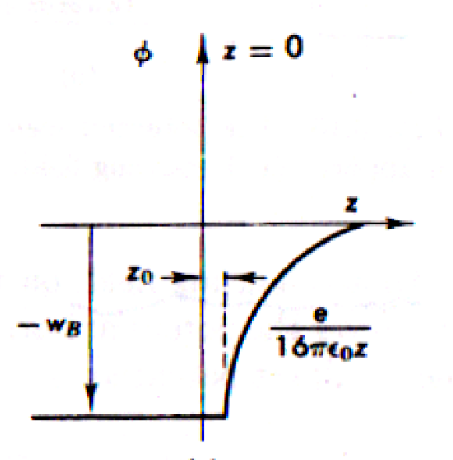
\includegraphics[width=0.7\linewidth]{../imagenes/pozo.png}
    \caption{Pozo de potencial en el material}
    \label{fig:1}
\end{figure}

\vspace{0.2 cm}
De esta manera, si al incrementar la temperatura del conductor es tal que la energía $E$ de sus electrones es mayor a $w_b$, estos podrán escapar del conductor. Asi, al ser liberados estos se encontraran alrededor del conductor formando una nube de electrones la cual se puede retirar mediante una fuerza eléctrica generando una corriente eléctrica proporcional a dicha fuerza.

\subsection{Ley de Child}
Asi, sea una placa metálica como la de la figura \ref{em1}, la cual se encuentra en $x<0$ y a su derecha, en $x>0$, se encuentra el vacío. A cierta distancia $b$, se encuentra un ánodo plano con potencial positivo $V_{a}$ tal que este atrae a los electrones \textit{'evaporados'} del cátodo hacía este ánodo.

\begin{figure}[H]
    \centering
    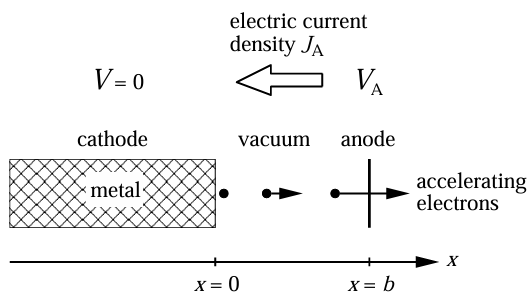
\includegraphics[width=0.8\linewidth]{../imagenes/Emisión termoiónica.png}
    \caption{Emisión termoiónica en un material conductor.}
    \label{em1}
\end{figure}

\vspace{0.2 cm}
Si $n(x)$ es la densidad de electrones en función de la distancia $x$ y $v(x)$ su velocidad se tiene entonces una densidad de corriente eléctrica de la forma:

\begin{align*}
    J(x) = en(x)v(x)
\end{align*}

\vspace{0.2 cm}
Suponiendo que los electrones se desprenden del metal con velocidad nula o casi nula a un potencial $V= 0$, entonces, se puede despejar la velocidad de la forma:

    \begin{align*}
        \frac{1}{2}mv(x)^{2} - eV(x) &= 0\\
        v(x) &= \sqrt{\frac{2e}{m}V(x)}.
    \end{align*}

\vspace{0.2 cm}
Donde $m$ es la masa del electrón.
\\

De esta manera, podemos plantear la ecuación de Poisson para los electrones en el vació ($0<x<b$) tal que:

\begin{align*}
    \nabla^{2}V &= -\frac{\rho (x)}{\varepsilon_{0}} \\ \Rightarrow \hspace{0.2 cm} \frac{\partial^{2}V}{\partial x^{2}} &= -\frac{en(x)}{\varepsilon_{0}} = \frac{J(x)}{\varepsilon_{0}\sqrt{\frac{2e}{m}V(x)}}
\end{align*}

\vspace{0.2 cm}
Y dado que el campo electrico debe ser cero en la superficie del material y los electrones se desprenden con velocidad nula, se tienen las condiciones de frontera:

\begin{align*}
    \left. \frac{\partial V}{\partial x}\right|_{x=0}&=0\\
        \left. V\right|_{x=0}&=0
\end{align*}

\vspace{0.2 cm}
Ahora, trasladando este problema a dos cilindros coaxiales de longitud $L$ y de radios $a$ y $b$ tal que $b>a$ :

\begin{figure}[H]
    \centering
    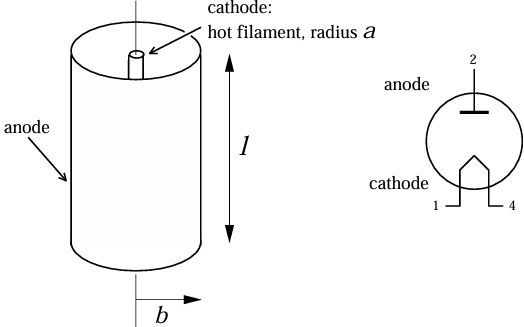
\includegraphics[width=0.8\linewidth]{../imagenes/Cilindros.png}
    \caption{Cilindros coaxiales formando un diodo en un tubo de vacio}
    \label{fig:2}
\end{figure}

\vspace{0.2 cm}
Se tiene la ecuación de Poisson en coordenadas cilindricas:

\begin{align}
    \label{poiscilin}
    \nabla^{2}V(r) = \frac{j}{2\pi r \varepsilon_{0}\sqrt{\frac{2e}{m}}} V(r)^{-1/2},
\end{align}

\vspace{0.2 cm}
Donde $j$ = $\frac{I}{L}$ es la densidad lineal de corriente. Solucionando la ecuación (\ref{poiscilin}) se obtiene la relación:

\begin{equation}
    J_{A}= \frac{4\varepsilon_{0}}{9r_{a}^{2}\beta^{2}}\sqrt{\frac{2e}{m}}V_{A}^{3/2}
    \label{eq: Ley de Child cilindrica}
\end{equation}


\vspace{0.2 cm}
La cual es la ley de Child para un diodo cilíndrico.

\subsection{Ley de Richardson}

Considérese un electrón rebotando dentro de una caja cuadrada de longitud $L$ con un vértice en el origen y el vértice diagonalmente opuesto en ($L,L,L$), por medio de la hipótesis de De Broglie podemos considerar una función de onda de la forma $\psi$ = $Ne^{i\Vec{k}\cdot\Vec{r}}$.
\\

Se sabe que el momento del electrón es $\Vec{p}$ = $\hbar\Vec{k}$, las condiciones de frontera periódicas de la caja requieren entonces que:

\begin{align*}
    k_i = \frac{2\pi n_i}{L}
\end{align*}

\vspace{0.2 cm}
Es decir, la función de onda esta definida por el vector $\vec{n}= (n_{x},n_{y},n_{z})$. Aplicando la ecuación de Schr\"odinger se encuentra que la energía asociada es:

\begin{align}
    \label{ecuan}
    E(\Vec{n)} = \frac{\hbar^{2}\vec{k}^{2}}{2m}= \frac{(2\pi\hbar)^{2}\vec{n}^{2}}{2mL^{2}}
\end{align}

\vspace{0.2 cm}
Igualando la expresión (\ref{ecuan}) a la energía cinética del electrón obtenemos su velocidad:

\begin{align*}
    \vec{v}= \frac{2\pi\hbar}{mL}\vec{n}
\end{align*}

\vspace{0.2 cm}
Podemos interpretar este último resultado como que las velocidades permitidas en lo estados cuánticos forman una red cúbica de lado $\frac{2\pi\hbar}{mL}$.
\\

Asi, para encontrar el número de estados de velocidades permitidas en una región especificada, dividimos volumen de dicha región sobre $(\frac{2\pi\hbar}{mL})^{3}$, es decir. Por lo tanto, el número de estados por volumen con velocidades entre $v$ y $v + \triangle v$ viene dado por la siguiente expresión:

\begin{align*}
    \frac{\triangle v_{x}\triangle v_{y}\triangle v_{z}}{(2\pi\hbar/m)^{3}}= \mathcal{N} \triangle v_{x}\triangle v_{y}\triangle v_{z}
\end{align*}

\vspace{0.2 cm}
De esta manera, definimos la constante de densidad de estados en el espacio de velocidades $\mathcal{N}$ de la forma:

\begin{align}
    \label{densidaddeestd}
    \mathcal{N} = \frac{1}{(2\pi\hbar/m)^{3}}
\end{align}

\vspace{0.2 cm}
Teniendo en cuenta esto, se sabe que el electrón es una partícula de spin 1/2, en consecuencia, la probabilidad de que un estado particular con energía $E$ viene dado por la distribución de Fermi-Dirac:

\begin{align*}
    f(E) = \frac{1}{1+e^{(\frac{E-E_{F}}{kT})}}
\end{align*}

\vspace{0.2 cm}
Y bajo la aproximación $E>>E_{F}$, se tiene:

\begin{align}
    f(E) \approx e^{-\frac{E-E_{F}}{kT}}
    \label{eq: Energía de Fermi}
\end{align}

\vspace{0.2 cm}
Donde $E_f$ se conoce como la energía de Fermi, este es el nivel mas alto de energía que pueden alcanzar los electrones en un pozo de potencial de profundidad $U$. En concordancia, definimos la función trabajo:

\begin{align*}
    W = U - E_f
\end{align*}

\begin{figure}[H]
    \centering
    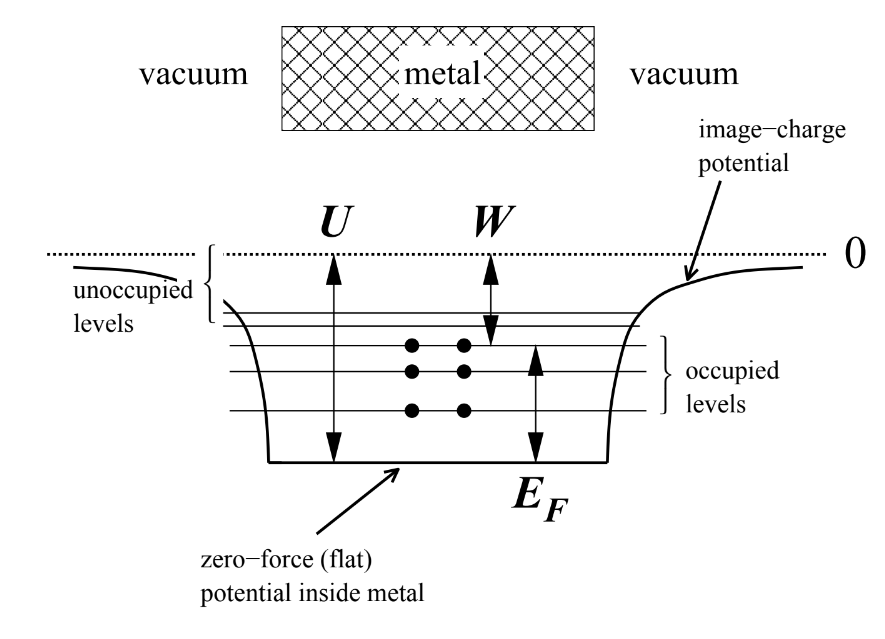
\includegraphics[width=0.8\linewidth]{../imagenes/fermi.png}
    \caption{Electrones en un metal bajo un pozo de potencial $U$. Los estados cuánticos posibles se llenan hasta el nivel de la energía de Fermi $E_f$.}
    \label{fig:3}
\end{figure}

\vspace{0.2 cm}
La cual se puede ver como la energía mínima requerida para liberar un electrón del pozo de potencial.
\\

Finalmente, se sabe  la probabilidad relativa de un evento que requiera energía $\Delta E$ en un sistema a temperatura absoluta $T$ es el factor de Boltzmann $e^{-\Delta E/kT}$. En este caso, un electrón requiere la energía de la función trabajo $\Delta E$ = $W$. 
\\

De esta manera, para que un electrón atraviese una sección de área transversal $\mathcal{A}$ en un intervalo de tiempo $\Delta t$ el electrón debe de estar a una distancia $v_{x}\Delta t$ y su velocidad debe de apuntar en dirección a la sección de área en cuestión.
\\

\begin{figure}[H]
    \centering
    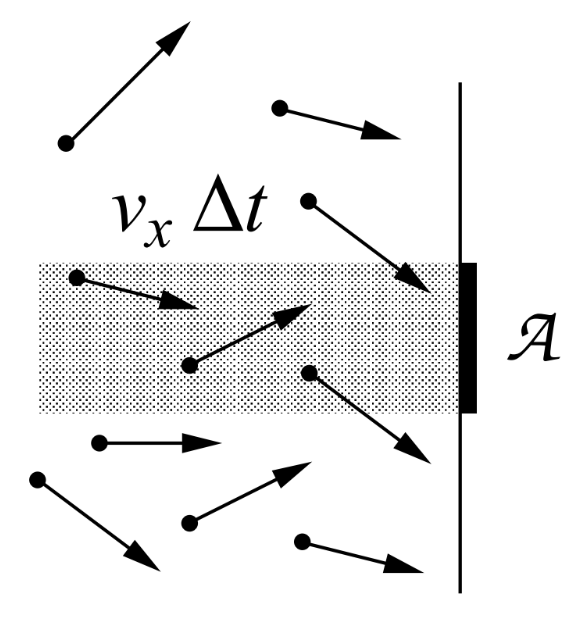
\includegraphics[width=0.5\linewidth]{../imagenes/Opera Captura de pantalla_2024-03-13_211045_mail.google.com.png}
    \caption{Electrones atravesando una sección de área $\mathcal{A}$}
    \label{fig:4}
\end{figure}

Mediante la densidad de estados (\ref{densidaddeestd}), la energía de Fermi (\ref{eq: Energía de Fermi}) y el factor de Boltzmann se puede obtener el número de electrones escapando por la sección de área $\mathcal{A}$ durante un tiempo $\Delta t$ mediante la siguiente expresión:

\begin{align*}
    J= \int_{-\infty}^{\infty} \int_{-\infty}^{\infty} \int_{\sqrt{2U/m}}^{\infty}\left[2\mathcal{N}f(E)Av_{x}\triangle t \right] dv_{x}dv_{y}dv_{z}
\end{align*}

\vspace{0.2 cm}
Resolviendo la integral se obtiene la ley de Richardson:

\begin{align*}
    J = AT^{2}e^{-\frac{W}{kT}}
\end{align*}

\vspace{0.2 cm}
Donde:

\begin{align*}
    A = \frac{4\pi e\cdot m \cdot k^{2}}{h^{3}} = 1.2\cdot 10^{6} \text{A/m}^{2}\text{k}^{2}
\end{align*}

\vspace{0.2 cm}
 Se conoce como la constante de Richardson.
\\

Sin embargo, cuando se aplica un campo electrico que acelera los electrones en dirección al ánodo, la profundidad del pozo de potencial $w_b$ se ve reducida. Por ende, la ley de Richardson queda de la forma:

\begin{equation}
    J=AT^2e^{-\frac{e(\Phi + V_0)}{kT}}=J_0e^{-\frac{V_0e}{kT}}
    \label{eq: Ley de Richardson}
\end{equation}

\vspace{0.2 cm}
Ahora, dado que el nuevo potencial que experimentan los electrones es:

\begin{align*}
    V=-\frac{e}{16\pi \epsilon_0 z}-\frac{V_0z}{d}
\end{align*}

\vspace{0.2 cm}
Se tiene un máximo tal que:

\begin{align*}
    V_{max}=-2\sqrt{\frac{eV_0}{16\pi \epsilon_0 d}},\ \text{en}\ z=\sqrt{\frac{ed}{16\pi \epsilon_0 V_0}}
\end{align*}

Entonces, la barrera de potencial que los electrones deben superar es de

\begin{align*}
    e\Phi=-V_{max}-w_b=-w_b+2\sqrt{\frac{eV_0}{16\pi \epsilon_0 d}}
\end{align*}

\vspace{0.2 cm}
Y en consecuencia, la corriente de saturación resultante es:

\begin{equation}
    J_s=J_0e^{0.44\frac{\sqrt{E}}{T}}
    \label{eq: Densidad corriente campo cero}
\end{equation}

\vspace{0.2 cm}
 Un detalle importante es que cuando el campo acelerador es muy fuerte, se disminuye la barrera de potencial y los electrones se liberan con mayor facilidad e incluso es posible que sea atravesada gracias al efecto túnel afectando así lo predicho por la ley de Richardson. A esto se le llama emisión de Schottky.

\subsection{Ley de Stefan-Boltzmann}

Partiendo de la ley de Planck, la cual describe la radiación electromagnética emitida por un cuerpo negro en equilibrio térmico en una temperatura definida. Esta se resume en la siguiente expresión:

\begin{align*}
    \rho_{T}(\lambda)d\lambda = \frac{8\pi h c}{\lambda^{5}}\frac{d\lambda}{e^{\frac{hc}{\lambda kT}}-1}
\end{align*}

\begin{figure}[H]
    \centering
    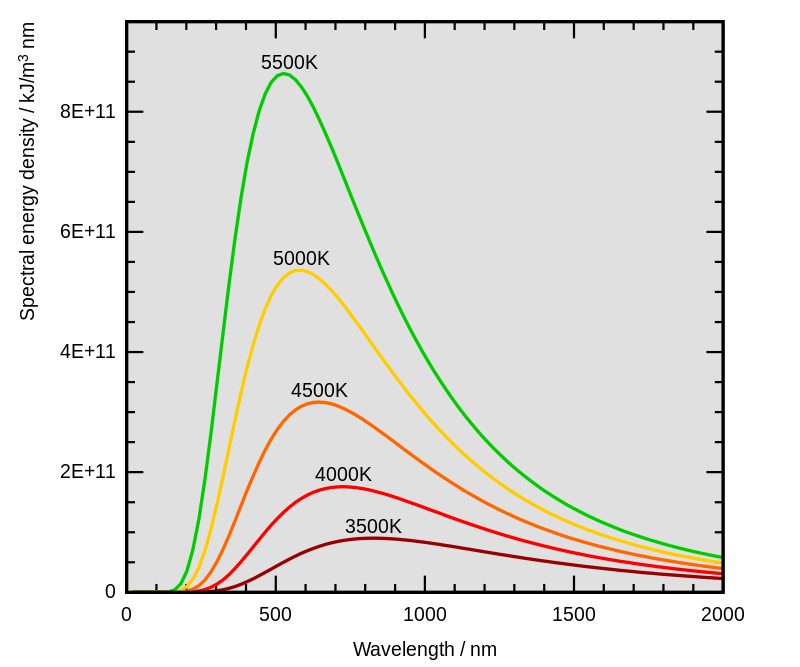
\includegraphics[width=0.8\linewidth]{../imagenes/Wiens_law.png}
    \caption{Ley de Planck para diferentes temperaturas.}
    \label{fig:5}
\end{figure}


\vspace{0.2 cm}
Donde $\rho_{T}(\lambda)$ representa la densidad de energía a cierta temperatura $T$ constante. Para obtener la radiancia total integramos la ley de Planck en todo el espectro:

\begin{align}
    \nonumber
    R_T &= \int_{0}^{\infty} \rho_{T}(\lambda) \mathrm{d}\lambda\\
    \boldsymbol{R_T} &\boldsymbol{= \sigma T^4}
    \label{eq: Ley de Stefan}
\end{align}


\vspace{0.2 cm}
Es decir, la energía total emitida de un cuerpo negro a temperatura $T$, donde $\sigma$ es la constante de Steffan-Boltzmann, de valor $5.67\cdot 10^{-5}$ W/m$^{2}$K$^{4}$.
\\

Teniendo en cuenta estas tres leyes respecto a la emisión termoiónica de un material conductor, se realizaran las medidas de las diferencias de potencial e intensidades de corriente eléctricas, junto con la temperatura del material conductor ,de tal forma que se puedan comprobar la relación funcional de la ley de Child, la ley de Richardson y la ley de Stefan-Boltzmann.

\section{Procedimiento Experimental}
En este sentido, para lograr el objetivo de esta practica experimental se llevo a cabo el siguiente montaje experimental:

\begin{figure}[H]
    \centering
    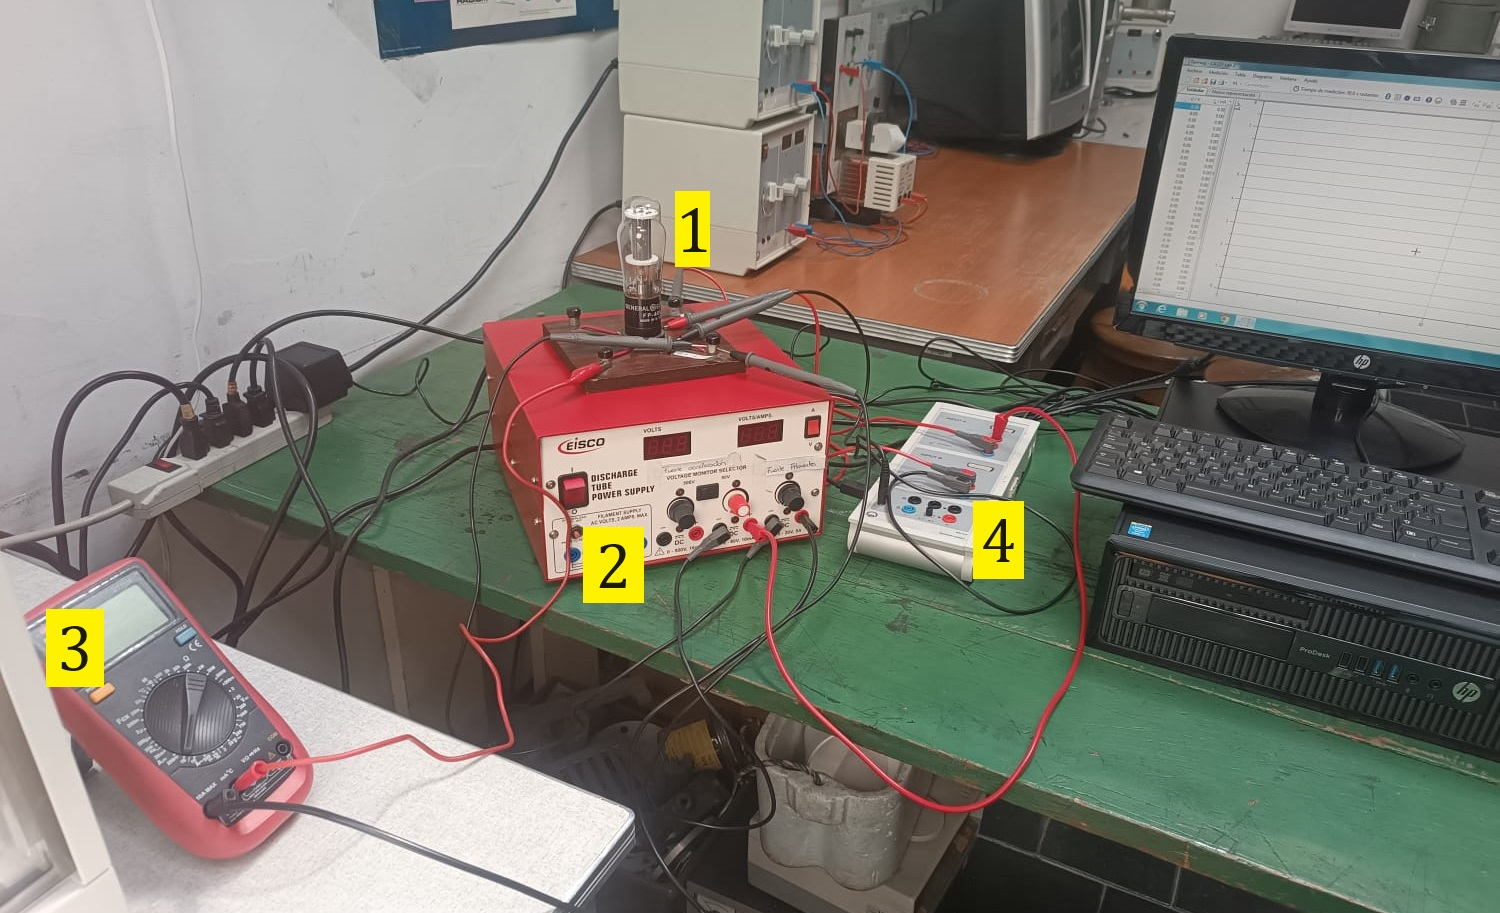
\includegraphics[width=0.9\linewidth]{../imagenes/MontajeEFM2nada.jpg}
    \caption{Montaje experimental}
    \label{montajel}
\end{figure}

En este podemos observar:

\begin{enumerate}[label=\textbf{\arabic*.}]
    \item \textbf{Tubo de vacio GE FP-400 \cite{fp400}:} Es un diodo cilindrico diseñado para ser utilizado en el estudio de descargas eléctricas en alto vacío. Consiste en un tubo de alto vacío con un filamento de tungsteno puro en su centro, ubicado axialmente en un ánodo cilíndrico recubierto de circonio-níquel. La resistividad del tungsteno a $27^{o}$ C es $(5.64 \pm 0.01)\cdot 10^{-6}$. Este cuenta con las dimensiones:

    \begin{itemize}
        \item Longitud (L) = $(3.17 \pm 0.01)$ cm
       \item  Diámetro filamento (2a) = $(0.013 \pm 0.001)\text{cm}$
        \item Diámetro ánodo (2b) = $(1.58 \pm 0.001)$ cm
        \item Máximo voltaje filamento = $(4.75 \pm 0.01)$ V
        \item Máxima corriente filamento = $(2.5 \pm 0.1)$ A
        \item Máximo voltaje ánodo = $(125 \pm 1)$ V
        \item Máxima corriente ánodo = $(0.055 \pm 0.001)$ A
        \item Máxima disipación ánodo = $(15 \pm 1)$ W
    \end{itemize}

    \item \textbf{Fuente de poder AC/DC marca Eisco Labs \cite{eisco}:} Suministra tres voltajes DC de salida independientes, proporcionando un voltaje alto (0 a 500V, 10mA y 0 a 80V, 10mA) y un voltaje bajo (0 a 20V, 5A), permitiéndose usar simultáneamente.

    \item \textbf{Dos (2) Multímetro digital modelo UT151 marca UNI-T \cite{unit}:} Se utilizara para medir los voltajes y corrientes del montaje experimental.

    \item \textbf{Sensor-CASSY 2 LB 524 013 \cite{sensorcassy}:} Consiste en un sistema de adquisición de datos que permite convertir señales analógicas en digitales para su registro y análisis en una computadora u otro dispositivo compatible.
\end{enumerate}
\begin{itemize}
    \item \textbf{Cables}
\end{itemize}



El circuito empleado para esta practica experimental es:
\\

\begin{figure}[H]
    \centering
    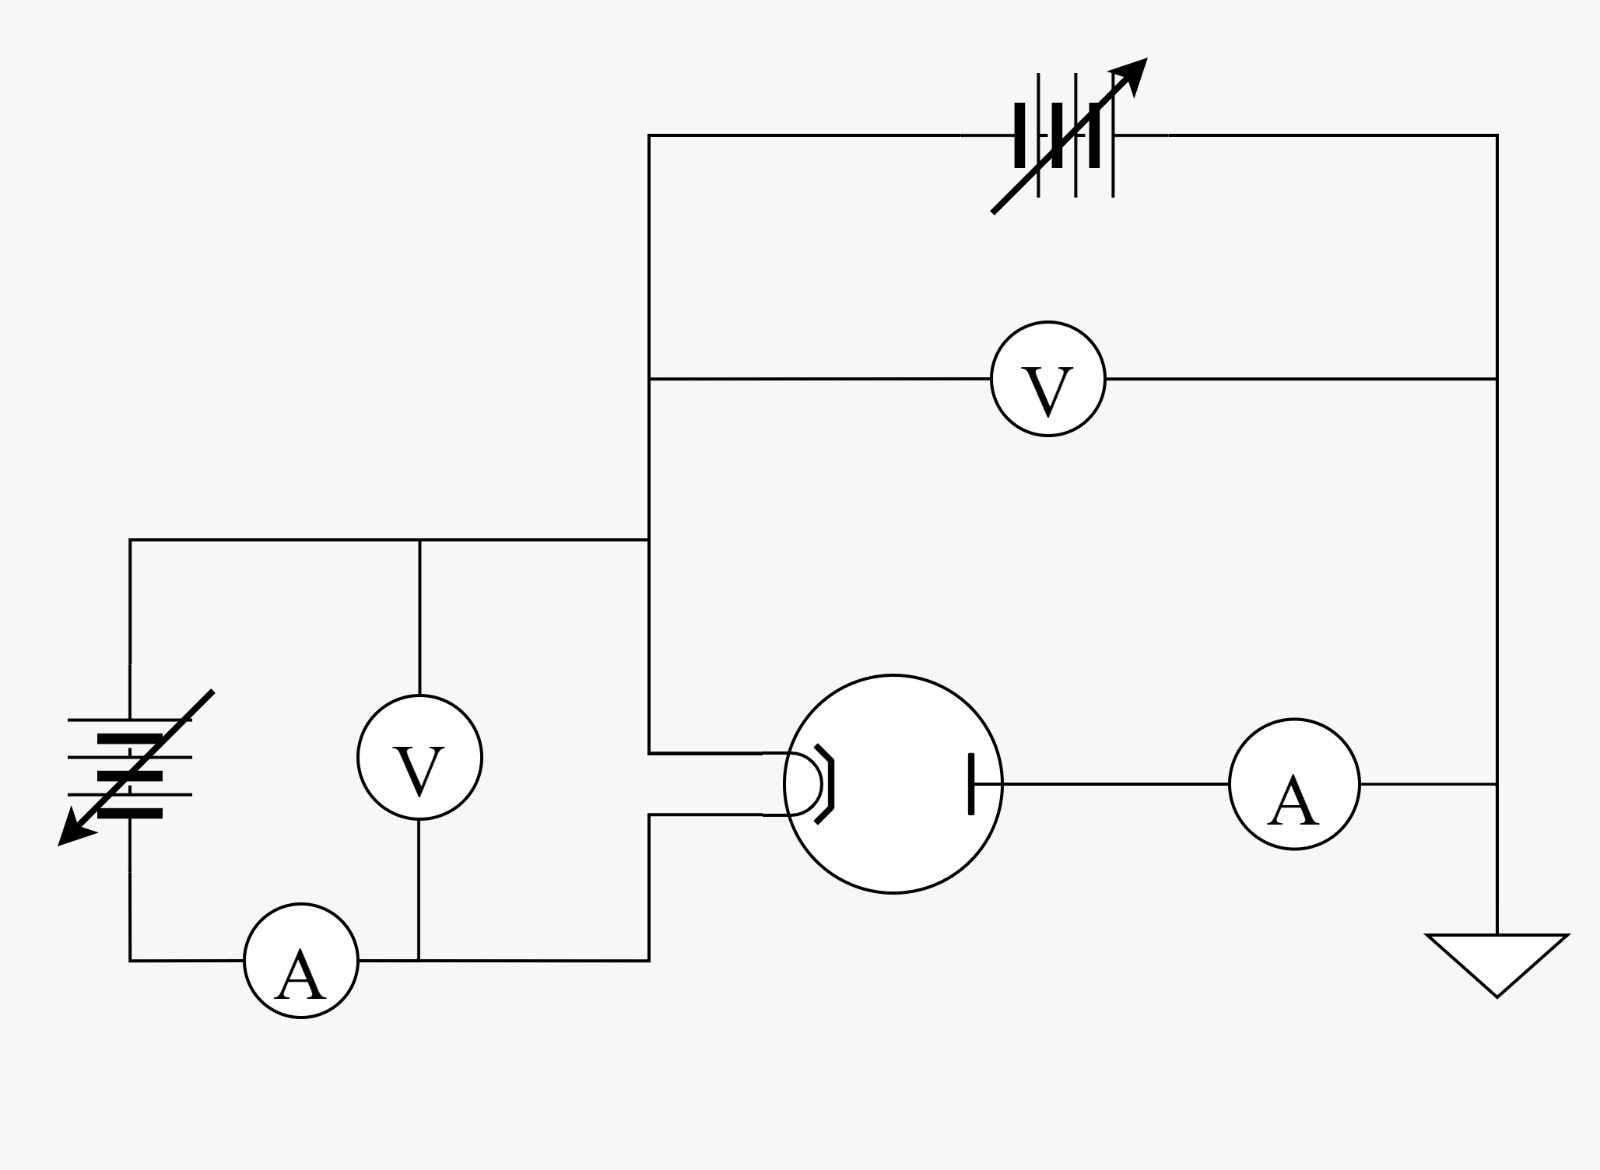
\includegraphics[width=0.8\linewidth]{../imagenes/circuito.jpeg}
    \caption{Circuito eléctrico compuesto por dos (2) amperímetros $A$, dos (2) voltímetros $V$, dos (2) fuentes de poder variables y un diodo de vacio FP 400.}
    \label{fig:6}
\end{figure}

Mediante el cual se puede determinar los voltajes y corrientes tanto en el cátodo como en el ánodo del diodo, sin embargo, también la temperatura del filamento de tungsteno, lo que involucra la compleja tarea de medir altas temperaturas en el vació, no se puede tener contacto directo con el material cuya temperatura se busca medir, lo que imposibilita la tarea de utilizar los métodos tradicionales para medirla (termómetros, termoresitores, etc.).
\\

Convenientemente, se sabe que la resistencia eléctrica es aproximadamente proporcional a la temperatura. Del trabajo de Jones y Langmuir \cite{jones} sobre filamentos de tungsteno, Kirkman encontró la formula:

\begin{equation}
    T_{r}(x) = 112 +202x -181x^2
    \label{eq: Kirkman}
\end{equation}
    
\vspace{0.2 cm}
Donde $x$ es la razon de la resistencia caliente y la resistencia a 273 K.
\\

De esta manera, al momento de medir la resistencia se medirá tanto la resistencia de los filamentos como la de los alambres que lo sostienen en el tubo de vació.

\begin{align*}
    R_{\text{medida}} = R_{\text{filamento}} + R_{\text{alambres}}
\end{align*}

Por lo que la resistencia del filamento de tungsteno es:

\begin{align*}
    R_{\text{filamento}} = R_{\text{medida}} - R_{\text{alambres}}
\end{align*}

\vspace{0.2 cm}
Ya que no se puede medir directamente la resistencia de los alambres (debido a la estructura del tubo de vació). No queda mas alternativa que definir la resistencia de los alambres como una constante  y así calcular la resistencia de los alambres a partir de un valor calculado para la resistencia del filamento a temperatura ambiente.
\\

Se sabe que para el tubo de vacio FP-400 en frío se tienen los valores $I$ = (54.3 $\pm$ 0.1) mA y $V$ = (11,6 $\pm$ 0.1) mV y para la resistencia del filamento en frió gracias al fabricante se conoce el valor de su resistencia en (0,135 $\pm$ 0.001) $\Omega$.
\\

Asi, se continuara suministrando una corriente al diodo de 1.8 A, aumentándola en pasos de aproximadamente 0.5 A hasta llegar a una corriente casi máxima de 2.2 A, mediante uno de los multímetros se comprobara el valor de la corriente.
\\

Una vez verificado el valor de la corriente, en cada paso se dejara alcanzar el equilibrio térmico del filamento (en pausas de aproximadamente 30 segundos) y luego se medirá el voltaje y la corriente a través del diodo mediante el segundo multimetro. Finalmente se determinara la temperatura del filamento por medio de la formula de Kirkman.
\\

Ademas, en cada uno de los pasos de corriente se recopilaran datos de (voltaje, corriente) del ánodo para cada valor de corriente, y por ende, temperatura constate del cátodo. Dando valores al voltaje del ánodo desde 0 V hasta 80 V se buscara comprobar mediante estos datos la ley de Child. Estos datos se registraran en un computador en intervalos de 30 segundos gracias al sensor-CASSY 2.

\section{Resultados y Discusión}

Los datos obtenidos de voltajes y corrientes tanto para el ánodo como para el cátodo, fueron pasados a un programa en Python tal que se pudiesen procesar los datos, realizar los cálculos necesarios, hallar las incertidumbres correspondientes y realizar ajustes a partir de estos datos. En cada cálculo realizado, se hallaron los valores de incertidumbre correspondientes mediante la forma general para el cálculo de incertidumbres (Véase el apéndice $\boldsymbol{A}$, específicamente la fórmula \ref{Itmbre_Varias_Medidas}). Para los ajustes de curva, se usó la función de ajuste de curva de la librería de Python \textit{Scipy}, la cual admite como parámetros las variables dependiente e independiente al igual que las incertidumbres de estas, tal que se obtuvieron los parámetros de la función en cuestión con sus correspondientes incertidumbres. Los datos de voltaje y corriente registrados en el filamento de tungsteno se encuentran en la tabla \ref{tab: V vs I filamento}.

\begin{table}[H]
    \centering
    \begin{tabular}{l|l||l|l}
        \toprule
        \toprule
        Corriente [A] & Voltaje [V] & Corriente [A] & Voltaje [V]\\
        \midrule
        1.80 $\pm$ 0.01  &  2.56 $\pm$ 0.01  & 2.05 $\pm$ 0.01  &  3.25 $\pm$ 0.01  \\
        1.80 $\pm$ 0.01  &  2.59 $\pm$ 0.01  & 2.05 $\pm$ 0.01  &  3.26 $\pm$ 0.01 \\
        1.85 $\pm$ 0.01  &  2.69 $\pm$ 0.01  & 2.10 $\pm$ 0.01  &  3.39 $\pm$ 0.01 \\
        1.85 $\pm$ 0.01  &  2.70 $\pm$ 0.01  & 2.10 $\pm$ 0.01  &  3.41 $\pm$ 0.01\\
        1.89 $\pm$ 0.01  &  2.82 $\pm$ 0.01  & 2.14 $\pm$ 0.01  &  3.53 $\pm$ 0.01 \\
        1.89 $\pm$ 0.01  &  2.83 $\pm$ 0.01  & 2.14 $\pm$ 0.01  &  3.53 $\pm$ 0.01 \\
        1.95 $\pm$ 0.01  &  2.99 $\pm$ 0.01  & 2.15 $\pm$ 0.01  &  3.55 $\pm$ 0.01\\
        1.96 $\pm$ 0.01  &  2.99 $\pm$ 0.01  & 2.16 $\pm$ 0.01  &  3.60 $\pm$ 0.01\\
        1.96 $\pm$ 0.01  &  3.00 $\pm$ 0.01  &  2.20 $\pm$ 0.01  &  3.68 $\pm$ 0.01 \\
        2.00 $\pm$ 0.01  &  3.13 $\pm$ 0.01  & 2.20 $\pm$ 0.01  &  3.69 $\pm$ 0.01  \\
        2.00 $\pm$ 0.01  &  3.13 $\pm$ 0.01  & & \\
        \bottomrule
        \bottomrule

    \end{tabular}
    \caption{Tabla de intensidades corriente y Voltajes en el ánodo.}
    \label{tab: V vs I filamento}
\end{table}

Para la comprobación de la Ley de Child, se realizará un análisis funcional del comportamiento de la corriente en función del voltaje en el ánodo. Se tomaron los datos de voltaje y corriente en el ánodo tales que presentasen comportamientos lineales, antes de que la corriente para cada caso tomase un valor constante. Se asume que los datos presentan un comportamiento potencial, dada las intuiciones dadas por la ley de Child para placas cilíndricas (\ref{eq: Ley de Child cilindrica}). De esta forma, mediante una gráfica logarítmica se busca determinar el valor de la potencia bajo la suposición previa, puesto que operar la función logarítmica sobre la ley de Child expresada en términos de la corriente eléctrica se tiene la siguiente expresión:

\begin{align*}
    Ln(I) = Ln\left(\frac{8\pi \varepsilon_{0}r_{c}L}{9r_{a}^{2}\beta^{2}} \sqrt{\frac{2e}{m}}\right) + \frac{3}{2}Ln(V)
\end{align*}

\vspace{0.2 cm}
De este modo, graficar la corriente eléctrica en función del voltaje en el ánodo permite obtener la potencia de la forma funcional, cuyo valor teórico dada la ley de Child es $\frac{3}{2}$. Tras haber realizado las transformaciones de las variables corriente y voltaje a sus formas logarítmicas, se realizó un ajuste lineal para cada conjunto de estos datos, habiendo restringido manualmente la zona de la gráfica en la cuál la ley de Child aplica, es decir, la región donde se presenta un comportamiento aproximadamente lineal no constante.En la tabla \ref{tab: Potencias Ley de Child} se evidencian los valores de la potencia en las gráficas logarítmicas para cada uno de los 21 conjuntos de datos de corrientes y voltajes en el ánodo para los distintos valores de corriente en el filamento.

%Quizas dejarla en el apéndice (?) cambiar columna dato por corriente filamento
\begin{table}[H]
    \centering
    \begin{tabular}{l|l||l|l}
        \toprule
        \toprule
            Corriente  & Potencia  & Corriente  & Potencia \\
            filamento [A] & mejor& filamento [A] & mejor\\
        \midrule
         1.80 $\pm$ 0.01  &  1.80  $\pm$ 0.08 & 2.00 $\pm$ 0.01  &  1.60  $\pm$  0.03\\
         1.80 $\pm$ 0.01  &  1.7  $\pm$  0.2 & 2.05 $\pm$ 0.01  &  1.57  $\pm$  0.02\\
         1.85 $\pm$ 0.01  &  2.1  $\pm$  0.1 & 2.05 $\pm$ 0.01  &  1.48  $\pm$  0.02\\
         1.85 $\pm$ 0.01  &  1.87  $\pm$  0.06 & 2.10 $\pm$ 0.01  &  1.46  $\pm$  0.01\\
         1.89 $\pm$ 0.01  &  1.70  $\pm$  0.04 & 2.10 $\pm$ 0.01  &  1.42  $\pm$  0.01\\
         1.89 $\pm$ 0.01  &  1.64  $\pm$  0.03 &  2.14 $\pm$ 0.01  &  1.47  $\pm$  0.01\\
         1.95 $\pm$ 0.01  &  1.64  $\pm$  0.03 & 2.14 $\pm$ 0.01  &  1.43  $\pm$  0.01\\
         1.96 $\pm$ 0.01  &  1.60  $\pm$  0.03 & 2.15 $\pm$ 0.01  &  1.482  $\pm$  0.009\\
         1.96 $\pm$ 0.01  &  1.41  $\pm$  0.02 & 2.16 $\pm$ 0.01  &  1.45  $\pm$  0.01\\
         2.00 $\pm$ 0.01  &  1.56  $\pm$  0.02 & 2.20 $\pm$ 0.01  &  1.44  $\pm$  0.01 \\
        2.20 $\pm$ 0.01  &  1.395  $\pm$  0.008 & & \\
    \bottomrule
    \bottomrule
    \end{tabular}
    \caption{Tabla de valor de la potencia de la Ley de Child para cada intensidad de corriente en el filamento.}
    \label{tab: Potencias Ley de Child}
\end{table}

Con los datos de la tabla II definimos como el valor central a su promedio de forma que

\begin{align*}
    p=\langle p\rangle=1.581\ \text{W}
\end{align*}

\vspace{0.2 cm}
Con incertidumbre hallada mediante $\ref{Itmbre_Varias_Medidas}$ tal que

\begin{align*}
    \Delta p=\frac{1}{N}\sqrt{(\Delta p_1)^2+...+(\Delta p_{21})^2}=0.01\ \text{W}
\end{align*}

\vspace{0.2 cm}
Se tiene entonces el resultado para la potencia

\begin{align*}
    p=(1.58\pm 0.01)\ \text{W}
\end{align*}

\vspace{0.2 cm}
El cual es cercano al valor teórico de 3/2 con un error del $5\%$. 

\vspace{0.2 cm}

Se procede a hallar el valor de la resistencia del filamento de tungsteno para los diferentes valores de corriente eléctrica en este. En primer lugar, se halla el valor de la resistencia del soporte del filamento mediante los datos brindados de corriente ($54.3 \pm 0.01$) mA, voltaje ($11.6 \pm 0.01$) mV y resistencia del filamento en frío ($0.135\pm 0.01$) $\Omega$. Por ley de Ohm, se obtuvo la resistencia total $R_{T}$, es decir, la suma de la resistencia de los soportes $R_{s}$ y la del filamento en frío $R_{f}$.

\begin{align*}
    R_{T} &= \frac{V_{f}}{I_{f}} \\
    R_{T} &= (0.214 \pm 0.008)\text{ $\Omega$}
\end{align*}

\vspace{0.2 cm}
Luego, la resistencia del soporte es la siguiente:

\begin{align*}
    R_{s} &= R_{T} - R_{f}\\
    R_{s} &=  (0.079 \pm 0.008)\text{ $\Omega$}
\end{align*}

\vspace{0.2 cm}
Este valor de resistencia del soporte se asume constante, de forma que la corriente, voltaje y temperatura del sistema no influencian sobre este valor. Para hallar la resistencia del filamento de tungsteno para cada par de corriente y voltaje en este, se procede de manera similar. Se halla mediante ley de Ohm la resistencia total y se le resta el valor de la resistencia del soporte. Los valores de la resistencia del filamento se encuentran en la tabla \ref{tab: Resistencias filamento}.
\\

Como se mencionó previamente, dada la fórmula de Kirkman (\ref{eq: Kirkman}) se tiene una relación entre la temperatura del filamento de tungsteno y su resistencia, de modo que al hallar el valor de la resistencia del filamento se puede determinar la temperatura del cátodo para cada pareja de corriente y voltaje en este. Recordemos que la fórmula de Kirkman esta en términos de una razón de resistencias, la cual en nuestro caso será el cociente entre las resistencias halladas para el filamento y la resistencia del filamento en frío, es decir, $(0.135 \pm 0.01)$ $\Omega$. Una vez halladas todas las razones de resistencias, se operó la fórmula de Kirkman, de modo que se obtuvieron las temperaturas para cada una de las corrientes y resistencias del filamento (Tabla \ref{tab: Resistencias filamento}).


%Quizas dejarla en el apéndice (?)
\begin{table}[H]
    \centering
    \begin{tabular}{l|l|l}
        \toprule
        \toprule
        Corriente [A] & Resistencia [$\Omega$] & Temperatura [K]\\
        \midrule
        1.80 $\pm$ 0.01 &  1.422 $\pm$ 0,009  &  (194 $\pm$ 1)  $\cdot$ 10 $^{1}$\\
        1.80 $\pm$ 0.01  &  1.439 $\pm$ 0,009  &  (196 $\pm$ 1)  $\cdot$ 10\\
        1.85 $\pm$ 0.01  &  1.454 $\pm$ 0,009  &  (198 $\pm$ 1)  $\cdot$ 10 $^{1}$\\
        1.85 $\pm$ 0.01  &  1.459 $\pm$ 0,009  &  (199 $\pm$ 1)  $\cdot$ 10 $^{1}$\\
        1.89 $\pm$ 0.01  &  1.492 $\pm$ 0,009  &  (203 $\pm$ 1)  $\cdot$ 10 $^{1}$\\
        1.89 $\pm$ 0.01  &  1.497 $\pm$ 0,009  &  (203 $\pm$ 1)  $\cdot$ 10 $^{1}$\\
        1.95 $\pm$ 0.01  &  1.533 $\pm$ 0,009  &  (208 $\pm$ 1)  $\cdot$ 10 $^{1}$\\
        1.96 $\pm$ 0.01  &  1.526 $\pm$ 0,008  &  (207 $\pm$ 1)  $\cdot$ 10 $^{1}$\\
        1.96 $\pm$ 0.01  &  1.531 $\pm$ 0,008  &  (208 $\pm$ 1)  $\cdot$ 10 $^{1}$\\
        2.00 $\pm$ 0.01  &  1.565 $\pm$ 0,008  &  (212 $\pm$ 1)  $\cdot$ 10 $^{1}$\\
        2.00 $\pm$ 0.01  &  1.565 $\pm$ 0,008  &  (212 $\pm$ 1)  $\cdot$ 10 $^{1}$\\
        2.05 $\pm$ 0.01  &  1.585 $\pm$ 0,008  &  (214 $\pm$ 1)  $\cdot$ 10 $^{1}$\\
        2.05 $\pm$ 0.01  &  1.590 $\pm$ 0,008  &  (215 $\pm$ 1)  $\cdot$ 10 $^{1}$\\
        2.10 $\pm$ 0.01  &  1.614 $\pm$ 0,008  &  (218 $\pm$ 1)  $\cdot$ 10 $^{1}$\\
        2.10 $\pm$ 0.01  &  1.624 $\pm$ 0,008  &  (219 $\pm$ 1)  $\cdot$ 10 $^{1}$\\
        2.14 $\pm$ 0.01  &  1.650 $\pm$ 0,008  &  (222 $\pm$ 1)  $\cdot$ 10 $^{1}$\\
        2.14 $\pm$ 0.01  &  1.650 $\pm$ 0,008  &  (222 $\pm$ 1)  $\cdot$ 10 $^{1}$\\
        2.15 $\pm$ 0.01  &  1.651 $\pm$ 0,008  &  (222 $\pm$ 1)  $\cdot$ 10 $^{1}$\\
        2.16 $\pm$ 0.01  &  1.667 $\pm$ 0,008  &  (224 $\pm$ 1)  $\cdot$ 10 $^{1}$\\
        2.20 $\pm$ 0.01  &  1.673 $\pm$ 0,008  &  (224 $\pm$ 1)  $\cdot$ 10 $^{1}$\\
        2.20 $\pm$ 0.01  &  1.677 $\pm$ 0,008  &  (225 $\pm$ 1)  $\cdot$ 10 $^{1}$\\
        \bottomrule
        \bottomrule
    \end{tabular}
    \caption{Tabla de resistencia y temperatura para cada valor de corriente en el filamento}
    \label{tab: Resistencias filamento}
\end{table}

\vspace{0.2 cm}
Se puede ilustrar en la gráfica \ref{fig: Gráfica de Voltaje vs Corriente ánodo} el comportamiento de la corriente eléctrica en función del voltaje en el ánodo para distintas temperaturas del filamento.

\begin{figure}[H]
    \centering
    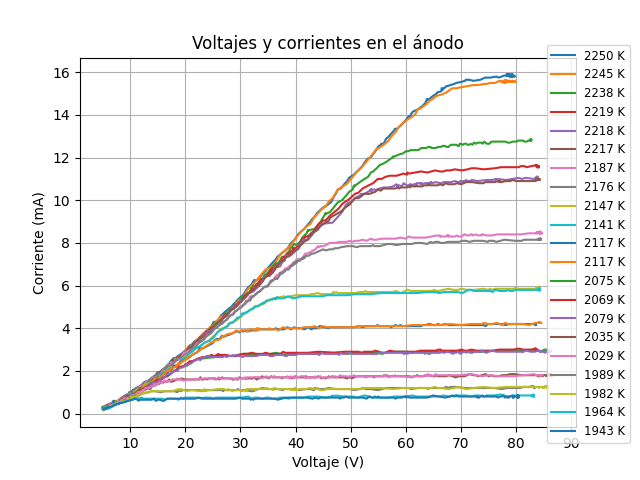
\includegraphics[width= 1\linewidth]{../graficas/Gráfica de Voltaje vs Corriente ánodo.png}
    \caption{Gráfica de intensidad de corriente en función del voltaje en el ánodo para cada temperatura medida.}
    \label{fig: Gráfica de Voltaje vs Corriente ánodo}
\end{figure}

\vspace{0.2 cm}
Mediante el producto del voltaje y la intensidad de corriente en el filamento, se halló la potencia eléctrica la cual se aproxima a la potencia de un cuerpo a temperatura $T$ con su factor de emisividad puesto que no se trata de un cuerpo negro. Los valores de la potencia se pueden ver en la tabla \ref{tab: Potencia eléctrica}.

\begin{table}[H]
    \centering
    \begin{tabular}{l|l||l|l}
        \toprule
        \toprule
        Temperatura [K] & Potencia [W] & Temperatura [K] & Potencia [W] \\
        \midrule
        (196 $\pm$ 2) $\cdot$ 10$^{1}$  &  4.61 $\pm$ 0.03 & (214 $\pm$ 1) $\cdot$ 10$^{1}$  &  6.26 $\pm$ 0.04 \\
        (198 $\pm$ 2) $\cdot$ 10$^{1}$  &  4.66 $\pm$ 0.03 & (215 $\pm$ 1) $\cdot$ 10$^{1}$  &  6.66 $\pm$ 0.04 \\
        (199 $\pm$ 2) $\cdot$ 10$^{1}$  &  4.98 $\pm$ 0.03 & (218 $\pm$ 1) $\cdot$ 10$^{1}$  &  6.68 $\pm$ 0.04\\
        (203 $\pm$ 1) $\cdot$ 10$^{1}$  &  5.00 $\pm$ 0.03 & (219 $\pm$ 1) $\cdot$ 10$^{1}$  &  7.12 $\pm$ 0.04\\
        (203 $\pm$ 1) $\cdot$ 10$^{1}$  &  5.33 $\pm$ 0.03 & (222 $\pm$ 1) $\cdot$ 10$^{1}$  &  7.16 $\pm$ 0.04\\
        (208 $\pm$ 1) $\cdot$ 10$^{1}$  &  5.35 $\pm$ 0.03 & (222 $\pm$ 1) $\cdot$ 10$^{1}$  &  7.55 $\pm$ 0.04 \\
        (207 $\pm$ 1) $\cdot$ 10$^{1}$  &  5.83 $\pm$ 0.04 & (222 $\pm$ 1) $\cdot$ 10$^{1}$  &  7.55 $\pm$ 0.04\\
        (208 $\pm$ 1) $\cdot$ 10$^{1}$  &  5.86 $\pm$ 0.04 & (224 $\pm$ 1) $\cdot$ 10$^{1}$  &  7.63 $\pm$ 0.04\\
        (212 $\pm$ 1) $\cdot$ 10$^{1}$  &  5.88 $\pm$ 0.04 & (224 $\pm$ 1) $\cdot$ 10$^{1}$  &  7.78 $\pm$ 0.04\\
        (212 $\pm$ 1) $\cdot$ 10$^{1}$  &  6.26 $\pm$ 0.04 & (225 $\pm$ 1) $\cdot$ 10$^{1}$  &  8.10 $\pm$ 0.04\\
        \bottomrule
        \bottomrule

    \end{tabular}
    \caption{Tabla de potencia eléctrica para las distintas temperaturas del filamento.}
    \label{tab: Potencia eléctrica}
\end{table}

\vspace{0.2 cm}
Recordando la forma funcional de la ley de Stefan-Boltzmann (ecuación \ref{eq: Ley de Stefan}), se aplica el logaritmo a esta ley, de forma que se tiene la siguiente igualdad:

\begin{align*}
    Ln(P) = Ln(\sigma) + 4Ln(T)
\end{align*}

\vspace{0.2 cm}
Se puede ver que el logaritmo de la potencia presenta un comportamiento lineal respecto al logaritmo de la temperatura, tal que al realizar un ajuste lineal en esta escala logarítmica, se obtiene que la pendiente de este ajuste es el valor del exponente de la temperatura en la ley de Stefan-Boltzmann. Se obtuvo que la pendiente de este ajuste lineal sobre las variables logarítmicas es $3.906 \pm 0.051$, como se puede ver en la gráfica.

\begin{figure}[H]
    \centering
    \includegraphics[width= 1\linewidth]{../graficas/Gráfica T vs P filamento.png}
    \caption{Gráfica en escala logarítmica de la potencia en función de la temperatura.}
    \label{fig: Gráfica T vs P filamento}
\end{figure}

\vspace{0.2 cm}
Para la ley de Richardson, deben de identificarse los valores de la corriente de saturación. Para ello, se definió manualmente para cada conjunto de datos de voltaje y corriente en el ánodo, un valor de voltaje a partir del cual el comportamiento de la intensidad de corriente respecto al voltaje es aproximadamente una constante, es decir, se toman aquellos datos correspondientes a la zona cuya tasa de crecimiento de voltaje es casi nula, precisamente donde se presenta la ley de Richardson que relaciona la corriente de saturación. Esta última se halla mediante el promedio de las intensidades de corriente correspondientes a la zona de datos filtradas para este fin. No en todas las gráficas se logra identificar la zona donde aplica la ley de Richardson, de forma que solo se tomaron las corrientes de saturación de ciertas gráficas. En la tabla \ref{tab: Corrientes de saturacion} se tienen las corrientes de saturación para los distintos valores de temperatura en las que fue posible registrar estos datos de corriente de saturación. 

\begin{table}[H]
    \centering
    \begin{tabular}{c|c}
        \toprule
        \toprule
        Temperatura [K)]& Corriente saturación [mA]\\
        \midrule
        (194 $\pm$ 2) $\cdot$ $10^{1}$  &  0.78 $\pm$ 0.04 \\
        (196 $\pm$ 2) $\cdot$ $10^{1}$  &  0.82 $\pm$ 0.04 \\
        (198 $\pm$ 2) $\cdot$ $10^{1}$  &  1.22 $\pm$ 0.04 \\
        (199 $\pm$ 2) $\cdot$ $10^{1}$  &  1.20 $\pm$ 0.04 \\
        (203 $\pm$ 1) $\cdot$ $10^{1}$  &  1.76 $\pm$ 0.04 \\
        (203 $\pm$ 1) $\cdot$ $10^{1}$ &  1.78 $\pm$ 0.04 \\
        (208 $\pm$ 1) $\cdot$ $10^{1}$  &  2.87 $\pm$ 0.04 \\
        (207 $\pm$ 1) $\cdot$ $10^{1}$  &  2.97 $\pm$ 0.05 \\
        (208 $\pm$ 1) $\cdot$ $10^{1}$  &  2.94 $\pm$ 0.03 \\
        (212 $\pm$ 1) $\cdot$ $10^{1}$  &  4.22 $\pm$ 0.04 \\
        (212 $\pm$ 1) $\cdot$ $10^{1}$  &  4.17 $\pm$ 0.04 \\
        (214 $\pm$ 1) $\cdot$ $10^{1}$  &  5.78 $\pm$ 0.05 \\
        (215 $\pm$ 1) $\cdot$ $10^{1}$  &  5.86 $\pm$ 0.03 \\

        \bottomrule
        \bottomrule

    \end{tabular}
    \caption{Tabla de corrientes de saturación.}
    \label{tab: Corrientes de saturacion}
\end{table}

\vspace{0.2 cm}
Dada la geometría cilíndrica del cátodo, se tiene que la densidad de corriente eléctrica viene dada por la siguiente expresión:

\begin{align*}
    J_{s}= \frac{I_{s}}{2\pi r_{c}L}
\end{align*}

\vspace{0.2 cm}
Por otro lado, dada la expresión \ref{eq: Densidad corriente campo cero} se tiene:

\begin{align*}
    J_{0} = J_{s}e^{-0.44\frac{\sqrt{E}}{T}}
\end{align*}

\vspace{0.2 cm}
Donde $E$ es el campo eléctrico, cuyo valor en este montaje es:

\begin{align*}
    E = \frac{V_{0}}{d},
\end{align*}

\vspace{0.2 cm}
 $V_{0}$ es la diferencia de potencial entre el cátodo y el ánodo, y $d$ es la distancia entre el cátodo y el ánodo. De esta forma, se obtuvieron los valores para la densidad de corriente para campo cero ($J_{0}$) mediante la siguiente expresión:
 
\begin{align*}
    J_{0}= J_{s}e^{-0.44\frac{\sqrt{V_{0}/d}}{T}}
\end{align*}

\vspace{0.2 cm}
Dada la ley de Richardson (\ref{eq: Ley de Richardson}), se tiene la siguiente igualdad:

\begin{align*}
    \frac{J_{0}}{T^{2}} = A_{0}e^{-e\phi / kT}
\end{align*}

\vspace{0.2 cm}
Aplicando logaritmo natural, se obtiene:

\begin{align*}
    Ln \left( \frac{J_{0}}{T^{2}} \right) = Ln(A_{0}) - \frac{e\phi}{k}\frac{1}{T}
\end{align*}

\vspace{0.2 cm}
Se puede evidenciar que hay un comportamiento lineal entre el logaritmo de la izquierda de la igualdad y el inverso de la temperatura. Del ajuste de curva, se tiene que la pendiente es igual a $-e\phi/k$, donde $e$ es la carga del electrón, $k$ es la constante de Boltzmann y $\phi$ es la función trabajo. Del ajuste de curva de la gráfica \ref{fig: Grafica Ley de Richardson}, se tiene que su pendiente es:

\begin{align*}
    -\frac{e\phi}{k} = (-3.9 \pm 0.1) \cdot 10^4 \text{ K}
\end{align*}

\vspace{0.2 cm}
Por consiguiente, el valor de la función trabajo es:

\begin{align*}
    \phi = (3.3 \pm 0.1)\text{ V}
\end{align*}

\begin{figure}[H]
    \centering
    \includegraphics[width= 1\linewidth]{../graficas/Gráfica JoT^-2 vs T^-1 semilog.png}
    \caption{Gráfica en escala semi-logarítmica de $J_{o}/T^{2}$ en función de $1/T$.}
    \label{fig: Grafica Ley de Richardson}
\end{figure}

\vspace{0.2 cm}
En cuanto a la razón entre la carga del electrón y su masa, esta se obtiene a partir de la relación entre la corriente de saturación y el voltaje de aceleración. Dicha expresión es la siguiente:

\begin{align}
    I_{s} = \frac{8\pi \varepsilon_{0}l}{9r_{a}\beta^{2}}\sqrt{2\frac{e}{m}}V_{0}^{3/2}
    \label{11}
\end{align}

\vspace{0.2 cm}
Puesto que los valores de corriente de saturación y el voltaje de aceleración son conocidos, luego, se realizó un ajuste a la función previa, de modo que se obtuvo el siguiente valor para la razón entre la carga y la masa:

\begin{align*}
    \frac{e}{m} = (1.3 \pm 0.4)\times 10^{13} \frac{\text{C}}{\text{kg}}
\end{align*}



\section{Conclusiones}

Con las mediciones realizadas se pudo obtener un valor de $(1.58\pm 0.01)\ \text{W}$ con un error del 5$\%$ respecto al valor teórico de 3/2 definido para el exponente en ($\ref{eq: Ley de Child cilindrica}$), siendo este un valor aceptable, se puede comprobar la validez de la  ley de Child para placas cilíndricas.
\\\\
Asimismo, al comparar el logaritmo natural de las temperaturas calculadas con la ley de Kirkman con el logaritmo de las potencias, la relación hallada fue una lineal que correspondía a la Ley de Stefan-Boltzmann con una pendiente de (3.91 $\pm$ 0.05) con un error del $2\%$ respecto al valor teórico de 4, considerando estos valores se pudo comprobar experimentalmente la ley de Stefan-Boltzmann para cuerpos grises.
\\

Para comprobar la ley de Richardson se encontró la relación entre el logaritmo natural de $J_0/T^2$ y el inverso de $T$, la cual es una recta con pendiente $-e\phi$/$k$. La pendiente hallada experimentalmente fue de $(-3.9 \pm 0.1) \cdot 10^4 \text{ K}$ con lo cual, tras despejar para la función trabajo $\Phi$ y reemplazar en ($\ref{11}$) encontramos la constante $e/m = (1.3 \pm 0.4) \times 10^{-13}$ C/kg del electrón que se aleja del valor teórico de $e/m = 1.79 \times 10^{11}$ C/kg \cite{codata}.
\\

Cualitativamente podemos notar comportamientos acordes a la emisión termoionica en la gráfica $\ref{fig: Gráfica de Voltaje vs Corriente ánodo}$, donde es claro que para mayor temperatura del cátodo, es mayor la corriente de saturación.
\\

Finalmente, para realizar los cálculos, sobre todo en la comprobación de la ley de Richardson, hubo una gran cantidad de datos y parámetros que fueron ajustados manualmente dando lugar a errores y a su propagación, provocando así resultados que distan de los valores teóricos en proporciones que nos indican que son erróneos aunque las formas funcionales coincidan con las teóricas.\\

Para los otros casos (Ley de Child y ley de Stefan-Boltzmann) la magnitud del error nos permite confirmar los resultados.


%\clearpage

\section{Apéndice}

\appendix
\section{Propagación de incertidumbres}
Sea una magnitud $x_i$ obtenida de forma directa mediante $N$ mediciones independientes teniéndose un error estándar del promedio $\sigma_{x_i}$. Si la incertidumbre nominal asociada a $x_i$ es $\sigma_{nom}$, su incertidumbre total es \cite{ardila}:

\begin{align*}
    \Delta x_i = \sqrt{(\sigma_{nom})^2+ (\sigma_{x_i})^2}
\end{align*}

\vspace{0.2 cm}
Por otro lado, sea una magnitud $\psi$ obtenida de forma indirecta a partir de los parámetros $x_{1}, x_{2}, \dotsb, x_{i}$ medidos directamente con incertidumbres $\Delta x_{1}, \Delta x_{2}, \dotsb, \Delta x_{i}$. La incertidumbre total de $\psi$, $\Delta \psi$ viene dada por la expresión \cite{ardila}:

\begin{align}
    \Delta \psi = \sqrt{\left( \frac{\partial \psi}{\partial x_{1}}\right)^2(\Delta x_{1})^2  + \dotsb + \left( \frac{\partial \psi}{\partial x_{i}}\right)^2(\Delta x_{i})^2}
    \label{Itmbre_Varias_Medidas}
\end{align}

\bibliography{report}

\end{document}
%
% ****** End of file apssamp.tex ******